\documentclass{beamer}

\usepackage{alltt}%
\usetheme{Boadilla}
\usecolortheme{seahorse}

\usepackage[utf8]{inputenc}
\usepackage{default}

\usepackage{xcolor}%for color mixing

\usepackage{amsmath}%
\usepackage{amsfonts}%
\usepackage{amssymb}%
\usepackage{graphicx}


\setbeamertemplate{itemize/enumerate body begin}{\small}


%%%%%%%%%%%%%%%%%%%%%%%%%%%%%%%%%%%%%%%%%%%%%%%%%%%%%%%%%%%%%%%%%%%%%%%%%%%%%%%%%%

\title{Statisitcal Thinking in Biology Research}
\author{Terry Neeman and Timothee Bonnet}
\date{\today}

\begin{document}

\begin{frame}{}
\maketitle

\end{frame}
%%%%%%%%%%%%%%%%%%%%%%%

\begin{frame}{Acknowledgemnts and warning}

\end{frame}
%%%%%%%%%%%%%%%%%%%%%%%

\begin{frame}{Key ideas for today}

\begin{itemize}[<+->]
 \item Statistics in biology is the study of biological variation
 \item Statistical ideas about biological variation inform the design of experiments
 \item Statistical ideas about biological variation inform the analysis of experiments
 \item Statistical thinking is an essential component of scientific thinking
\end{itemize}

\end{frame}
%%%%%%%%%%%%%%%%%%%%%%%

\begin{frame}{Cautionary tales from the front}

\end{frame}
%%%%%%%%%%%%%%%%%%%%%%%

\begin{frame}{Message 1: A small p-value is not always evidence of a treatment effect}

  \begin{columns}
    \begin{column}{0.5\textwidth}
	\begin{center}
	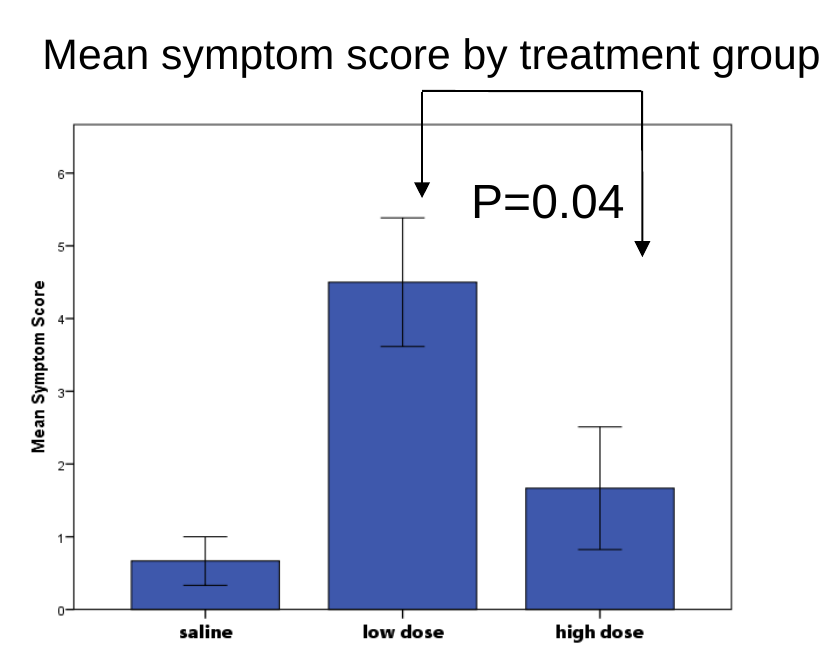
\includegraphics[width=\textwidth]{Figures/message1}
	\end{center}
    \end{column}
    
    \begin{column}{0.5\textwidth}
    \begin{block}{Vaccine challenge experiment:}
      \begin{itemize} 
       \item 6 mice/group (saline/low dose/high dose)
       \item All mice challenged with Shigella
       \item Followed for 14 days
       \item  Outcome: Symptom score average Days 2 - 8
      \end{itemize}
      \end{block}
      
      \begin{alertblock}{}
       One-way ANOVA (post-hoc Bonferroni) p=0.04
      \end{alertblock}

    \end{column}
  \end{columns}
  
  \pause \vspace{0.3cm}
  \emph{\large Do you think the vaccine works? What is strange?}
  

\end{frame}
%%%%%%%%%%%%%%%%%%%%%%%

\begin{frame}{Message 1: A small p-value is not always evidence of a treatment effect}
 \vspace{-0.2cm}
 \begin{center}
  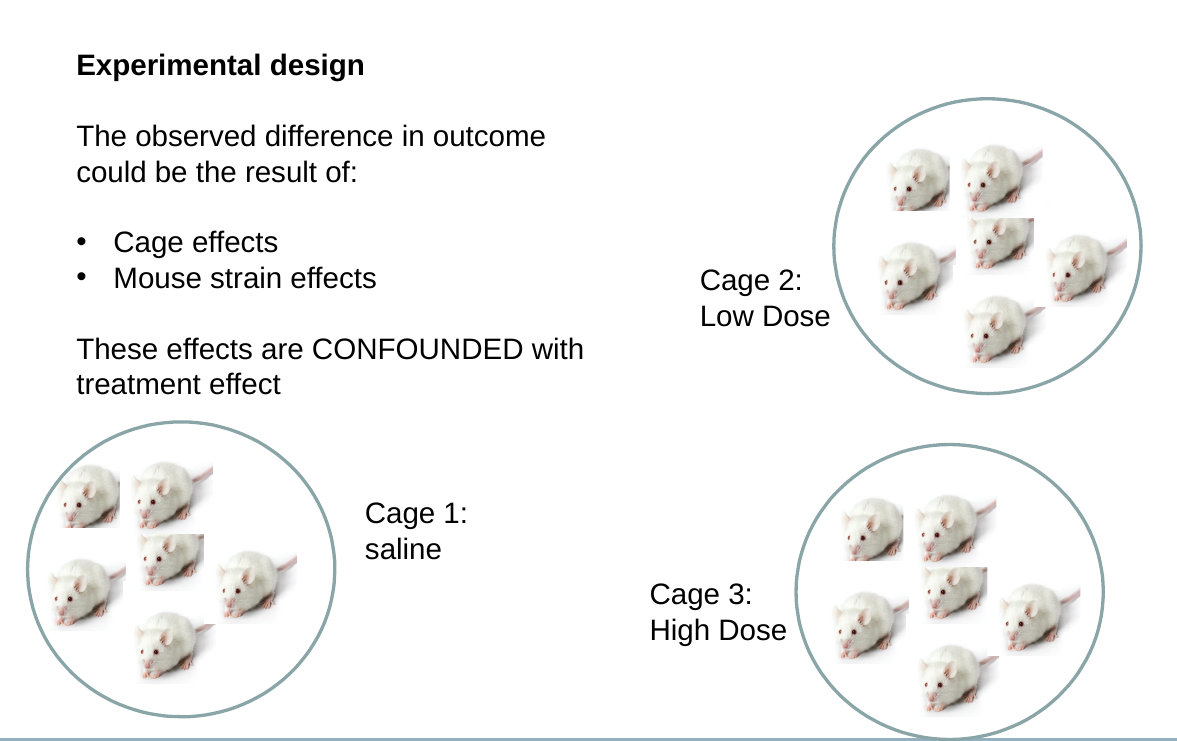
\includegraphics[width=\textwidth]{Figures/mice}
 \end{center}
 
\end{frame}
%%%%%%%%%%%

\begin{frame}{Message 2: p-values from simple comparisons cannot tell us when differences are “different”}
 
  \begin{columns}
    \begin{column}{0.5\textwidth}
	\begin{center}
	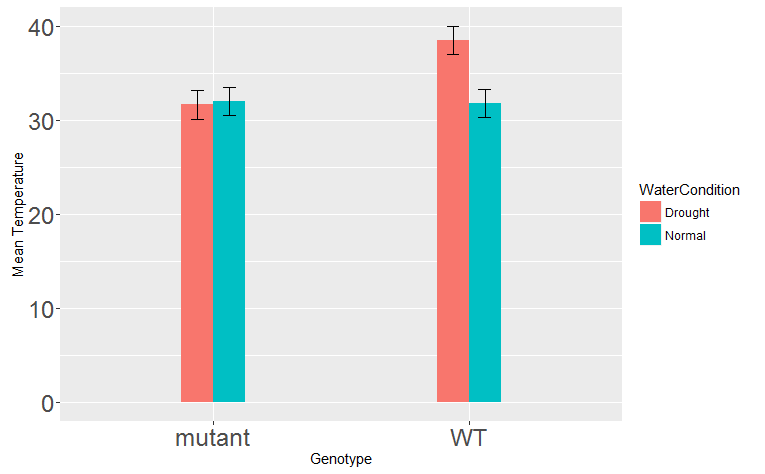
\includegraphics[width=\textwidth]{Figures/message2}
	\end{center}
    \end{column}
    
    \begin{column}{0.5\textwidth}
    \begin{block}{Are temperature mechanisms modified in a genetically modified tomato plant?}
      \begin{itemize}
	\item Genotypes: WT/mutant 
	\item Water condition: Normal/Drought
	\item Leaf temperature measured
      \end{itemize}
      \end{block}
  
    \end{column}
  \end{columns}
   
   
   \begin{alertblock}{Comparisons made using t-tests}
Evidence of difference + No evidence of difference $\neq$ Evidence that differences are different.
      \end{alertblock}
      
      
\end{frame}
%%%%%%%%%%%


\end{document}
